%   %==========================================================================
%   %  Comment
%   %==========================================================================
    \begin{mycomment}
        物体の運動を解析するとは,物体の運動軌跡や速度変化など数値的に把握するために
        計算することをいう.そのためには,ニュートンの運動方程式をつかう.
        この章では,運動方程式を使った運動の解析方法を,典型的な具体例を通して学習する.
    \end{mycomment}

%   %==========================================================================
%   %  Section
%   %==========================================================================
    \section{運動の解析方法}
        物体の運動を解析するには,以下の手順で行う.
        \begin{enumerate}
            \item 解析対象となる物体にかかるすべての力を書き出す
            \begin{itemize}
                \item 物体の運動方向が予めわかっているなら,垂直方向と平行方向に分解もする
            \end{itemize}
            \item 物体の質量を測る
            \item 物体の位置を未知変数として,ニュートンの運動方程式をたてる
            \item 運動方程式を解く
            \item 解をグラフ化,あるいは映像化して,具体的な運動のイメージを得る
        \end{enumerate}

%   %==========================================================================
%   %  Section
%   %==========================================================================
    \section{重要な例}
%       %======================================================================
%       %  SubSection
%       %======================================================================
        \subsection{等速直線運動}
            ニュートンの運動の第一法則である \textbf{慣性の法則} によれば,
            物体には,力が働かないときは,速度を変化させることなく
            動き続ける,という性質がある.速度を変化させることがないことを,
            \textbf{等速度} という
                \footnote{
                    速度が変化しないということは,
                    ずっと同じ速度を保っているのと同じこと.
                }.
            速度は,向きと大きさ(速さ)をもったベクトルである.だから,等速度で
            運動し続けるということは,向きと速さが常に一定であるということだ.
            向きが変わらないという事は,直線的な運動を続けるということ.
            このような運動を \textbf{等速直線運動} という.
            また,等速直線運動は,物体の慣性のみで運動していることから,
            \textbf{慣性運動} ということもある.

            ニュートンの運動の第二法則である,運動方程式からもこの性質を
            導ける.運動方程式は,以下のような形をしていた.
                \begin{equation*}
                    m \frac{{\df}^{2} \br}{{\df t}^{2}} = \bF.
                \end{equation*}
            $m$ は質量,$\br$ は位置,$t$ は時間,$\bF$ は力である.

            慣性の法則の仮定から,物体には力が働いていないので,$\bF=\bzero$ である.
            よって,慣性運動している物体の運動方程式は,
                \begin{align}
                    m \frac{{\df}^{2} \br}{{\df t}^{2}} = \bzero.
                \end{align}
            この運動方程式を質量 $m(>0)$ で割れば,等速直線運動の加速度を得る.
                \begin{align}
                    \frac{{\df}^{2} \br}{{\df t}^{2}} = \bzero.
                \end{align}
            等速直線運動では,加速度は $\bzero$,つまり,加速していないという結果が出た
                \footnote{
                    当たり前な結果で,何の面白みもないが,経験と理論の一致をここで見ることができる.
                }.
            言い方を変えれば,力が全く加わっていない物体は加速しない,とも言える.

            加速度を時間 $t$ で積分(不定積分)すると,速度 $\bv(t)$ が得られる.
                \begin{align*}
                    \bv(t) &= \int \left( \frac{{\df}^{2} \br}{{\df t}^{2}} \right) \df t  \\
                           &= \int \frac{\df}{\df t}\left( \frac{\df \br}{\df t}  \right) \df t  \\
                           &= \int \bzero \df t  \\
                           &= {\bv_{0}}.
                \end{align*}
                        改めて書きなおして,
                \begin{align}\label{eq:tousoku_chokusen_undou000}
                    \bv(t) = {\bv_{0}}.
                \end{align}

            ここで,左辺の積分定数を $\bv_{0}$ とした.$\bv_{0}$ は速度を示す一定のベクトルである.
            この値は,物体に力が働かなくなった瞬間の速度とみなせる.等速直線運動が開始された
            時刻の速度であり,特にこの速度を,\textbf{初速度} とよばれる.
            このことから,力の加えられていない物体は,一定速度で運動し続けることが確認された.

            さらに式(\ref{eq:tousoku_chokusen_undou000})を $t$ で積分して,
            位置 $x(t)$ を示す式を導出しておこう.
                \begin{equation*}
                   \bx(t) := \int {\bv_{0}} \df t =  {\bv_{0}} t +  {\bx_{0}}.
                \end{equation*}
            清書して,
                \begin{align}
                   \bx(t) =  {\bv_{0}} t +  {\bx_{0}}.
                \end{align}

            ここで,$\bx_{0}$ は位置を示す一定のベクトルである.
            この値は,物体に力が働かなくなった瞬間の位置とみなせる.等速直線運動が開始された
            時刻の位置であり,\textbf{初期位置} という.


%       %======================================================================
%       %  SubSection
%       %======================================================================
        \subsection{等加速度運動}
            物体に一定の力を与え続けると,物体はどうのように運動するだろうか.
            この場合の運動方程式は,ニュートンの運動方程式そのもので,
                \begin{equation*}
                    m \frac{{\df}^{2} \br}{{\df t}^{2}} = \bF.
                \end{equation*}
            この式の質量 $m$ はスカラー定数であり,力 $\bF$ は一定ベクトルである.
            両辺を $m$ でわって,定数を右辺に集中させておこう.
                \begin{equation*}
                    \frac{{\df}^{2} \br}{{\df t}^{2}} = \frac{\bF}{m}.
                \end{equation*}
            時間 $t$ で積分すれば,速度 $\bv(t)$ が求まる.式変形が煩雑にならないように,
            右辺と左辺を別々に計算しよう
                \footnote{
                    本当のところは,左辺の式変形はあまり興味がない.左辺の計算は,
                    この積分計算で,速度を計算できることを確認するためだけに計算される.
                    この計算の本命は,右辺の計算で,速度がどのように表されるかがわかる.
                }.
                \begin{align*}
                    \mbox{(左辺)}  &= \int \frac{{\df}^{2} \br}{{\df t}^{2}} \df t \\
                                    &= \int \frac{\df}{\df t}\left( \frac{\df \br}{\df t} \right) \df t \\
                                    &= \frac{\df \br}{\df t}.
                \end{align*}
                \begin{align*}
                    \mbox{(右辺)}  &= \int \frac{\bF}{m} \df t \\
                                    &= \frac{\bF}{m} t + {\bv}_{0}.
                \end{align*}
            右辺の計算で,最後に現れた ${\bv}_{0}$ は積分定数である.
            これは $t=0$ における物体の速度である(すぐ後で,右辺の次元を確認する).
            よって,
                \begin{align}
                    \bv(t) := \frac{\df \br}{\df t} = \frac{\bF}{m}  t.
                \end{align}
            念の為,左辺の次元が速度([m/s])になる確認しておこう.
            [$F$] = [kg m/s${}^{2}$],[m] = [kg],[t]=[s] であるので,
                \begin{equation*}
                    \frac{\mathrm{kg}\quad\mathrm{m/{s}^{2}}}{\mathrm{kg}} \mathrm{s} = \frac{\mathrm{m}}{\mathrm{s}}.
                \end{equation*}
            よって,上式の最右辺は速度の次元である.$\bF/m$ は加速度であるから
                \footnote{
                    次元を確認するまでもない.$m\ba=\bF$ から,直ちに $\ba=\bF/m$ がわかる.
                },
                \begin{equation*}
                    \ba := \frac{\bF}{m}
                \end{equation*}
            上記から,加速度が時間によらず一定であることが見て取れる.それゆえ,このような物体の運動を,
            \textbf{等加速度運動} という.

            以上から,等加速度運動の速度の式が得られた.
                \begin{align}
                    \bv(t) = \ba t + {\bv}_{0}.
                \end{align}

            位置の式は,この速度の式をさらに $t$ で積分することで得られる.
                \begin{align}
                    \frac{\df \br}{\df t} =  \ba t + {\bv}_{0}
                \end{align}
            を基にして,
                \begin{align*}
                    \mbox{(左辺)} &= \int \frac{\df \br}{\df \bt} \df t = \br.
                \end{align*}
                \begin{align*}
                    \mbox{(右辺)} &= \int \left( \ba t + {\bv}_{0} \right) \df t \\
                                   &= \int \ba t \df t + \int {\bv}_{0} \df t     \\
                                   &= \frac{1}{2}\ba {t}^{2} + {\bv}_{0} t + {\bx}_{0}.
                \end{align*}
            右辺の計算で,最後に現れた ${\bx}_{0}$ は積分定数であり,$t=0$ での位置(初期位置)を示す.
            以上から,等加速度運動の位置の式は,以下となる.
                \begin{align}
                    \bx(t) = \frac{1}{2}\ba {t}^{2} + {\bv}_{0} t + {\bx}_{0}.
                \end{align}

%       %======================================================================
%       %  SubSection
%       %======================================================================
        \subsection{等速円運動}\label{subsec:tousoku_enundou}
%           %==================================================================
%           %  SubsubSection
%           %==================================================================
            \subsubsection{はじめに}
                運動方程式の使い方の別の例として,等速円運動を考えてみよう.
                \textbf{等速円運動} とは,速さが一定で,軌道が円であるような
                物体の運動のことである.
                        \begin{figure}[hbt]
                            \begin{center}
                                \includegraphicsdefault{tousokuenundou.pdf}
                                \caption{等速円運動}
                                \label{fig:tousokuenundou}
                            \end{center}
                        \end{figure}

                軌道円は2次元で表現できるので,軌道円の存在する面に $x\,$--$\,y$ 座標を
                とろう.軌道円の中心に,座標の原点 O にとる.軌道円の半径を $r$ とし,
                物体の質量を $m$,速さ(速度ではない)を $v$ とする.

                本来は,運動方程式を記述し,これを解くことで軌道がわかるのであるが,今から
                行おうとしていることは,その逆である.今回は軌道と,その他のパラメータ
                (速度 $v$ の仮定など)を先に決めてしまい,これを満たすような運動方程式を探す
                ということをすることになる.今は円運動を記述するような運動方程式を知らず,
                わかっているのは,結果である.結果から原因を探るのは何かおかしい気がするが,
                どのような運動方程式になるかを知るには,これが一番の近道であると思う.以下
                の学習で得られる等速円運動の方程式は,惑星の運動
                    \footnote{
                        惑星は楕円軌道を描く事が知られられいるので,これは近似になってしま
                        うが,地球など,太陽に近い惑星は,ほとんど円軌道を描いていると考え
                        ても大した間違いではない.
                    }
                など,一般にも通用するものである.ということで,円運動の方程式はどのような
                形で表されるのか,以下で,導いていくことにしよう.

                さて,運動方程式を記述したいのだが,それには物体に働く力と,物体に生じてい
                る加速度を知る必要がある.以下で,順を追って確認していこう.


%           %==================================================================
%           %  SubsubSection
%           %==================================================================
            \subsubsection{角速度}
                ニュートンの運動方程式の一般的な形は $m(\df^{2}\br/\df t^{2})=\bF$ である.
                $m$ は単なるスカラーであることから,加速度 $\df^{2}\br/\df t^{2}$ の方向と,
                力 $\bF$ の方向は同じである.つまり,加速度と力のどちらか一方の
                方向が分かれば,他方も同じ向きであると言える.今回は,加速度の
                方向を調べていこう.

                加速度の方向は,図形的に見つけることができる.加速度は,
                速度の時間変化によって定義されるから,速度の変化を見てみればよい.
                速度が微小変化したとき,その変化の方向を考えればよいのだ.
                図を描いて考えてみよう.
                    \begin{figure}[hbt]
                        \begin{tabular}{cc}
                            \begin{minipage}{0.5\hsize}
                                    \begin{center}
                                                \includegraphicsdouble{tousokuenundou_kasokudo.pdf}
                                                \label{fig:tousokuenundou_kasokudo}

                                        (a)
                                    \end{center}
                            \end{minipage}
                            \begin{minipage}{0.5\hsize}
                                    \begin{center}
                                        \includegraphicsdouble{enundou_kasokudo.pdf}
                                        \label{fig:enundou_kasokudo}

                                        (b)
                                    \end{center}
                            \end{minipage}
                        \end{tabular}
                                \caption{等速円運動の加速度の向き}
                    \end{figure}

                物体の速度の変化を考えて,2つの異なる時刻の速度ベクトルを描いた($\bv$ と $\bv'$).
                この2つの速度ベクトルを平行移動して,始点を重ねて見ると,物体が等速円運動するときに
                変化しているのは,図の $\theta$ であることがわかる.いま,等速運動を考えているので,
                この $\theta$ は時間 $t$ に比例している,と考えられる.
                    \begin{equation*}
                        \theta \propto t.
                    \end{equation*}
                ここで比例定数 $\omega$ を用いると,
                    \begin{align}
                        \theta = \omega t
                    \end{align}
                と書ける.回転の速さは,角 $\theta$ の変化によって,記述できる.
                ということは,
                この式の $\omega$ によって,回転の速さを表していると見ることができる
                    \footnote{
                        時間の変化は測定する事ができず,常に一定であると考えるしかないので,
                        $\theta$ の時間変化が大きいということは,$\omega$ が大きいということになる.
                    }.
                そこで,$\omega$ は \textbf{角速度} とよばれる.実際,$\theta$ を時間微分すると,
                    \begin{align}
                        \omega = \frac{\df \theta}{\df t}
                    \end{align}
                となり,これは,ちょうど位置の時間変化
                    \begin{equation*}
                        v = \frac{\df x}{\df t}
                    \end{equation*}
                と同じ形をしている.

                改めて,角速度を定義しておく.
                    \begin{myshadebox}{角速度の定義}
                        角速度 $\omega$ は,次式で定義される.
                        \begin{align}
                            \omega := \frac{\df \theta}{\df t}
                        \end{align}
                    \end{myshadebox}

                \begin{memo}{速度と加速度は直交する(図形的説明)}
                    等速ということを仮定しているので,速度ベクトルの大きさは
                    常に一定である.従って,図の三角形は,二等辺三角形である.
                    この二等辺三角形の底辺の角を,$\phi$ で表すことにしよう.
                    この角度 $\phi$ は,一時的に使用するもので,物理的に特に
                    意味のあるものではないので,特別な名前はない.しかし,
                    この $\phi$ は速度ベクトルと加速度ベクトルとが作る角であり,
                    これからの考察で,重要な結果を導く.

                    三角形の内角の和は,${180\,}^{\circ}$ であるから,
                        \begin{equation*}
                            \phi + \phi + \omega t = {180\,}^{\circ}
                        \end{equation*}
                    である.この式の左辺の $(\theta =) \omega t$ は微少時間を考えれば,
                    $t\rightarrow 0$ のようになり,微少時間の間に,次式が成立する.
                        \begin{equation*}
                            \lim_{t\rightarrow 0} \{\phi + \phi + \omega t\} = 2\phi
                        \end{equation*}
                    つまり,$2\phi = {180\,}^{\circ}$ となって,
                        \begin{align}
                            \phi = {90\,}^{\circ}
                        \end{align}
                    である.

                    先に指摘した通り,この $\phi$ は速度ベクトルと加速度ベクトルとが,
                    交わって作る角である.つまり,
                        \begin{equation*}
                            \mbox{等速円運動では,速度と加速度は直交する.}
                        \end{equation*}
                    のである.
                    加速度が生じているのは,速度ベクトルの始点の部分と同じなので,
                    加速度ベクトルを平行移動して,図\ref{fig:enundo_sokudo_kasokudo}のように
                    する.
                            \begin{figure}[hbt]
                                \begin{center}
                                    \includegraphicsdefault{enundo_sokudo_kasokudo.pdf}
                                    \caption{等速円運動における,速度と加速度の関係}
                                    \label{fig:enundo_sokudo_kasokudo}
                                \end{center}
                            \end{figure}

                    速度ベクトルと直交することと,これまでに描いた図から分かるように,
                    加速度の向きは,物体から円の中心に向うかう向きである.物体は
                    軌道円上を常に移動しているので,加速度も向きも絶えず変化している.
                \end{memo}


%           %==================================================================
%           %  SubsubSection
%           %==================================================================
            \subsubsection{角速度と円の方程式}
                等速円運動のもう1つの仮定を思い出そう.軌道が円を描くことである.
                円を表す方程式を思い起こそう.それは,
                    \begin{equation*}
                        x^{2} + y^{2} = \mathrm{const} ( = r^{2} )
                    \end{equation*}
                である
                    \footnote{
                        const はconstantの省略で,一定値をとるという意味.
                        今の場合,半径の二乗($r^{2}$)に
                        相当する.ここで言いたいのは,一定値を取るということなので,
                        $r^{2}$ を括弧書きにした.あくまで参考と考えて欲しい.
                    }.
                図\ref{fig:tousokuenundou}をもう一度見て,確認のこと.
                もちろん用いている座標は,2次元直交座標である.
                これは三平方の定理を考えれば,当然のことである.
                今回は半径として $r$ をとっているので,軌道円の方程式は
                    \begin{align}\label{eq:en_no_houteisiki}
                        x^{2} + y^{2} = r^{2}
                    \end{align}
                となる.
                        \begin{figure}[hbt]
                            \begin{center}
                                \includegraphicsdefault{en_no_houteisiki.pdf}
                                \caption{円の方程式}
                                \label{fig:en_no_houteisiki}
                            \end{center}
                        \end{figure}

                さて,三角関数の公式に次のようなものがある.
                    \begin{equation*}
                        \sin^{2}\theta + \cos^{2}\theta = 1.
                    \end{equation*}
                少し唐突に感実かもしれないが,実は,これは,円と関係がある.
                この公式は,図形的に解釈すると,
                半径が1で,$x=\sin\theta$,$y=\cos\theta$ の
                円の方程式と,考えられるからである.
                この公式を,(\ref{eq:en_no_houteisiki})に形を近づけてみよう.
                両辺に $r^{2}$ をかけて,$\theta$ を $\omega t$ に書き換える.
                \begin{equation*}
                    r^{2}\sin^{2}(\omega t) + r^{2}\cos^{2}(\omega t) = r^{2}.
                \end{equation*}
                つまり,
                \begin{align}
                    \left( r\sin( \omega t )\right)^{2} + \left( r\cos( \omega t ) \right)^{2} = r^{2}
                \end{align}
                である.この式は
                    \begin{align}
                        \begin{cases}
                        \displaystyle x(t) = r\cos( \omega t ) \\
                        \displaystyle y(t) = r\sin( \omega t ) \\
                        ( \mbox{半径} ) : r
                        \end{cases}
                    \end{align}
                の「円の方程式」である.これが,今回考える軌道円の方程式である.

%           %==================================================================
%           %  SubsubSection
%           %==================================================================
            \subsubsection{等速円運動の速度と加速度の導出}
                さて,軌道円の方程式が得られ,物体の軌道を直交座標で表すことができた.
                速度の定義は,直交座標では位置 $x(t)$ の時間微分 $\df x/\df t$ であった.従って,
                上で得た位置 $x(t)$,$y(t)$ の式を時間 $t$ で微分すれば,各方向の速度を求められる.
                やってみよう.ただし,三角関数の微分は,ここでは,既に知っているものと,仮定する
                    \footnote{
                        三角関数の微分公式
                            \begin{equation*}
                                \frac{\df }{\df x} \sin x = \cos x
                            \end{equation*}
                            \begin{equation*}
                                \frac{\df }{\df x} \cos x = -\sin x
                            \end{equation*}
                        合成関数 $f\{g(x)\}$ の微分($f(y)$,$y=g(x)$ とおく)
                            \begin{equation*}
                                \frac{\df}{\df x}f\{g(x)\} = \frac{\df g(x)}{\df x} \frac{\df f(y)}{\df y}
                            \end{equation*}
                    }.

                まず,$x$ 座標の速度 $v_{x}(t) = \df x /\df t$は($r$ は半径(定数))
                    \begin{align*}
                        \frac{\df}{\df t} r\cos(\omega t)
                            &= r\frac{\df (\omega t)}{\df t}\frac{\cos(\omega t)}{\df (\omega t)} \notag \\
                    \notag \\
                        \therefore\quad
                            v_{x}(t) &= -r\omega \sin(\omega t)
                    \end{align*}
                $y$ 座標の速度 $v_{y}(t) = \df y /\df t$は
                    \begin{align*}
                        \frac{\df}{\df t} r\sin(\omega t)
                            &= r\frac{\df (\omega t)}{\df t}\frac{\sin(\omega t)}{\df (\omega t)} \notag \\
                    \notag \\
                        \therefore\quad
                            v_{y}(t) &= r\omega \cos(\omega t)
                    \end{align*}

                また,加速度は,速度の微分であり,
                まず,$x$ 座標の速度 $a_{x}(t) =\df v_{x} / \df t$は
                    \begin{align*}
                        \frac{\df}{\df t} \{-r\omega \sin(\omega t)\}
                            &= -r\omega\frac{\df (\omega t)}{\df t}\frac{\sin(\omega t)}{\df (\omega t)} \notag \\
                    \notag \\
                        \therefore\quad
                            a_{x}(t) &= -r\omega^{2} \sin(\omega t)
                    \end{align*}
                $y$ 座標の速度 $a_{y}(t) = \df v_{y} /\df t$は
                    \begin{align*}
                        \frac{\df}{\df t} \{r\omega \cos(\omega t)\}
                            &= r\omega\frac{\df (\omega t)}{\df t}\frac{\cos(\omega t)}{\df (\omega t)} \notag \\
                    \notag \\
                        \therefore\quad
                            a_{y}(t) &= -r\omega^{2} \sin(\omega t)
                    \end{align*}

                結果をまとめておこう.
                    \begin{myshadebox}{等速円運動の速度と加速度の公式}
                        等速円運動は平面上の運動なので,2次元で表現できる.
                        等速円運動をする物体の位置 $\br(t)$ 速度 $v(t)$,加速度 $\ba(t)$ は次の
                        通りである
                            \footnote{
                                記号が紛らわしくなってしまった.ここでいう位置 $\br = (\, x(t) , \, y(t)\,)$ と
                                半径 $r$ は全く別のものであるので注意してほしい.
                            }.
                        \begin{align}
                            \br(t) &= \left( x(t) , \, y(t) \right) \notag \\
                                   &= \left( r\cos(\omega t),\, r\sin(\omega t) \right)
                        \end{align}
                        \begin{align}
                            \bv(t) &= \left( v_{x}(t) , \, v_{y}(t) \right) \notag \\
                                   &= \left( -r\omega \sin(\omega t),\, r\omega \cos(\omega t) \right)
                        \end{align}
                        \begin{align}
                            \ba(t) &= \left( a_{x}(t) , \, a_{y}(t) \right) \notag \\
                                   &= \left( -r\omega^{2} \cos(\omega t) ,\, -r\omega^{2} \sin(\omega t) \right)
                        \end{align}
                    \end{myshadebox}


%           %==================================================================
%           %  SubsubSection
%           %==================================================================
            \subsubsection{等速円運動の位置と速度と加速度の関係}
                今得られた等速円運動の位置 $\br(t)$ 速度 $v(t)$,加速度 $\ba(t)$ は,見るからに,
                互いに関係があることが察せられる.ここで次に,その関係を整理しよう.

                まず,位置 $\br(t)$ と加速度 $\ba(t)$ の関係を調べる.位置を表す式
                    \begin{align*}
                        \begin{cases}
                        \displaystyle x(t) = r\cos( \omega t ) \\
                        \displaystyle y(t) = r\sin( \omega t )
                        \end{cases}
                    \end{align*}
                    と加速度を表す式
                    \begin{align*}
                        \begin{cases}
                        \displaystyle a_{x}(t) = -r\omega^{2} \cos(\omega t) = -\omega^{2}( r \cos(\omega t) )\\
                        \displaystyle a_{y}(t) =-r\omega^{2} \sin(\omega t) = -\omega^{2} ( r \sin(\omega t) )
                        \end{cases}
                    \end{align*}
                を見比べよう.加速度の式の中に,位置の関数が現れている.
                つまり,位置と加速度の間に,以下の関係式を得る.
                    \begin{myshadebox}{等速円運動の位置と加速度との関係}
                        等速円運動する物体の位置と加速度の関係は,次式で表される.
                        \begin{align}
                            \begin{cases}
                            \displaystyle a_{x}(t) = -\omega^{2} x.\\
                            \displaystyle a_{y}(t) = -\omega^{2} y.
                            \end{cases}
                        \end{align}
                    \end{myshadebox}


                特に,加速度の大きさだけが知りたい場合,
                    \begin{align*}
                        |\ba| = a &= \sqrt{ {a_{x}}^{2}  +  {a_{y}}^{2} }   \\
                                    &= \sqrt{ {(-\omega^{2}x)}^{2}  +  {(-\omega^{2} y)}^{2} }  \\
                                    &= \sqrt{ \omega^{4}x^{2} + \omega^{4}y^{2} } \\
                                    &= \omega^{2} \sqrt{x^{2} + y^{2} } \\
                                    &= r\omega^{2} \;,\quad ( r = \sqrt{ x^{2} + y^{2} } )
                    \end{align*}
                と計算される.
                    \begin{myshadebox}{等速円運動の位置と加速度の大きさとの関係}
                        等速円運動する物体の,加速度の大きさをだけを考える場合,以下の式が
                        成立している.
                            \begin{align}
                                    a = r\omega^{2}.
                            \end{align}
                    \end{myshadebox}

                次に,位置と速度の関係を調べる.位置を表す式
                    \begin{align*}
                        \begin{cases}
                        \displaystyle x(t) = r\cos( \omega t ) \\
                        \displaystyle y(t) = r\sin( \omega t )
                        \end{cases}
                    \end{align*}
                と速度を表す式
                    \begin{align*}
                        \begin{cases}
                        \displaystyle v_{x}(t) = -r\omega \sin(\omega t) = -\omega r\sin(\omega t) \\
                        \displaystyle v_{y}(t) = r\omega \cos(\omega t)  = \omega r\cos(\omega t)
                        \end{cases}
                    \end{align*}
                を見比べよう.つまり,位置と速度の間に,以下の関係式を得る.
                    \begin{myshadebox}{等速円運動の位置と速度との関係}
                        等速円運動する物体の位置と速度の関係は,次式で表される.
                        \begin{align}
                            \begin{cases}
                            \displaystyle v_{x}(t) = -\omega y. \\
                            \displaystyle v_{y}(t) = \omega  x.
                            \end{cases}
                        \end{align}
                    \end{myshadebox}

                $x$ 座標と $y$ 座標が入れ替わっていること注意しよう.

                    特に,速度の大きさだけが知りたい場合,
                    \begin{align*}
                        |\bv| = v &= \sqrt{ {v_{x}}^{2}  +  {v_{y}}^{2} }   \\
                                    &= \sqrt{ {(-\omega y)}^{2}  +  {(\omega x)}^{2} }  \\
                                    &= \sqrt{ \omega^{2}y^{2}  +  \omega^{2}x^{2} } \\
                                    &= \sqrt{ \omega^{2} ( x^{2}  +  y^{2}) } \\
                                    &= \omega\sqrt{ x^{2}  +  y^{2} }\\
                                    &= r\omega \;,\quad ( r = \sqrt{ x^{2} + y^{2} } )
                    \end{align*}
                と計算される.
                    \begin{myshadebox}{等速円運動の位置と速度の大きさとの関係}
                        等速円運動する物体の,加速度の大きさをだけを考える場合,以下の式が
                        成立している.
                            \begin{align}
                                    v = r\omega.
                            \end{align}
                    \end{myshadebox}

            等速円運動の特徴は,後に確認する「単振動」という現象にも現れる.
            単振動は波動現象の解析の基礎である.量子力学によれば,
            原子レベルの微小なスケールで考えれば,物質には“物質波”という
            波動の性質をもっていることを,受け入れざるを得なくなる.
            これは素粒子理論にもつながる重要な現象である.

                \begin{memo}{速度と加速度は直交する(演繹的説明)}
                    最後に速度と加速度の関係を求めよう.
                    速度と加速度の関係は特に重要である.この関係から,
                    等速円運動において,速度ベクトルと加速度ベクトルが直交することが
                    導かれるのである.次の計算を見て欲しい.

                        今までに計算して位置と加速度,位置と速度の関係をもう一度書くと,
                            \begin{align*}
                                \begin{cases}
                                \displaystyle a_{x}(t) = -\omega^{2}x \\
                                \displaystyle a_{y}(t) = -\omega^{2} y \\
                                \displaystyle v_{x}(t) = -\omega y \\
                                \displaystyle v_{y}(t) = \omega x
                                \end{cases}
                            \end{align*}
                        である.

                        ベクトルの内積を思い出そう.ここでは,成分が分かっているので,
                        代数的な内積の計算方法を使う.

                        速度ベクトル $\bv(t)$ と加速度ベクトル $\ba(t)$ の内積をとると,
                            \begin{align*}
                                \bv(t) \cdot \ba(t) &= v_{x}(t)a_{x}(t) + v_{y}(t)a_{y}(t) \\
                                                    &= ( -\omega y ) ( -\omega^{2}x ) + ( \omega x ) ( -\omega^{2} y ) \\
                                                    &= \omega^{3}xy - \omega^{3}xy
                            \end{align*}
                            \begin{align}
                                \therefore\quad
                                \bv(t) \cdot \ba(t) = 0.
                            \end{align}
                        つまり,ベクトルの内積の性質より,速度ベクトル $\bv(t)$ と加速度ベクトル $\ba(t)$ は
                        直交すると言える.これは上で図を用いて確認したことと,同じ結果を得る.
                    \end{memo}


%           %==================================================================
%           %  SubsubSection
%           %==================================================================
            \subsubsection{円運動の周期と角速度}
                    等速円運動する物体が一回転する時間を,\textbf{周期} という.
                    周期の記号は大文字の $T$ がよく用いられる.このノートでも $T$ をつかう.
                    角速度 $\omega$ を用いて,周期 $T$ を表そう.

                    半径 $r$ の円の,周囲の長さは $2\pi r$ である.
                    つまり,円を一周するということを,$2\pi r$ だけ変位すると
                    言い換えられる.物体はこの円の上を
                    速さ $v$ で運動するから,$2\pi r$ だけ移動するのに掛かる時間,
                    つまり,物体の周期を $T$ とすれば,
                        \begin{equation*}
                            vT = 2\pi r.
                        \end{equation*}
                    つまり,
                        \begin{equation*}
                            T  =  \frac{2\pi r}{v}
                        \end{equation*}
                    である.等速円運動の場合,$v=r\omega$ が成立していることを上で確認している.
                    これを上式に代入すると,
                        \begin{equation*}
                            T = \frac{2\pi r}{r\omega} = \frac{2\pi}{\omega}
                        \end{equation*}
                    となる.

                    以上をまとめておこう.
                    \begin{myshadebox}{速度と周期と角速度の関係}
                        等速円運動の周期 $T$ と角速度 $\omega$ のには次の関係式が
                        成立する.
                        \begin{align}
                            T  =  \frac{2\pi r}{v}  =  \frac{2\pi }{\omega}.
                        \end{align}
                    \end{myshadebox}


%           %==================================================================
%           %  SubsubSection
%           %==================================================================
            \subsubsection{等速円運動の運動方程式}
                    加速度を得ることができたので,これで等速円運動を表現する
                    運動方程式をつくれる.運動方程式は,成分で書くと,
                        \begin{align*}
                            \begin{cases}
                            \displaystyle m\frac{\df^{2} x}{\df t^{2}} = F_{x} \\
                            \displaystyle m\frac{\df^{2} y}{\df t^{2}} = F_{y}
                            \end{cases}
                        \end{align*}
                    だから,これに今得られた加速度を代入して,
                        \begin{align}
                            \begin{cases}
                            \displaystyle mr\omega^{2} \cos(\omega t) = -F_{x} \\
                            \displaystyle mr\omega^{2} \sin(\omega t) = -F_{y}
                            \end{cases}
                        \end{align}

%   %==========================================================================
%   %  Section
%   %==========================================================================
    \section{地球重力下での運動}
%       %======================================================================
%       %  SubSection
%       %======================================================================
        \subsection{理想的な地球の形}
            以下でそれぞれの速度を計算するんだけど,その際に注意すべきことは,
            現実の地球そのものを想像してほしくない,ということ.
            表現の簡略化するために,「地球」という言い方をするが,この場合の地球は,
            現実の地球と同じ半径で,同じ質量をもった球をイメージしてもらいたい.
            ここで考える地球は大気の存在しない,のっぺらぼうな球である.

            \begin{memo}{計算で使う記号}
                計算の際に使用する記号を,書いておく.

                                \begin{tabular}{ll}
                                        $G$       [Nm${}^{2}$/s${}^{2}$] &: 万有引力定数($6.673 \times 10^{-11}$ )\\
                                        $R_{E}$   [m] &: 地球の半径  ($6.378 \times 10^{6}$   )                    \\
                                        $M_{E}$   [kg] &: 地球の質量  ($5.974 \times 10^{24}$  )                   \\
                                        $M_{S}$   [kg] &: 太陽の質量  ($1.989 \times 10^{30}$  )                   \\
                                        $D_{E-S}$ [m] &: 太陽と地球の距離($1.496 \times 10^{11}$  )                      \\
                                        $U_{E}$    &: 地球の重力の位置エネルギー                                     \\
                                        $m$        &: 物体の質量                                                   \\
                                        $h$        &: 地表からの鉛直方向の距離   %\\
                                    \end{tabular}
                上記の添字で, $E$ は地球(Earth),$S$ は太陽(Sun) の頭文字である.括弧内の値は,それぞれの具体的な数値.
            \end{memo}



%       %======================================================================
%       %  SubSection
%       %======================================================================
        \subsection{地表の重力加速度}
            式(\ref{eq:GravAccer000})にて,惑星の重力加速度を定義した.
            \begin{equation*}
                \textit{\textbf{g}} :=
                G\frac{M_{P}}{{\left| \br \right|}^{2}}
                \frac{\br}{\left| \br \right|} \quad (\mbox{(式(\ref{eq:GravAccer000})に同じ)}).
            \end{equation*}

            この式に,惑星の質量 $M_{P}$ に,地球の質量 $M_{E}$ を当てはめれば,
            そのまま地球の重力加速度となる.
                \begin{equation*}
                    \textit{\textbf{g}} :=
                    G\frac{M_{E}}{{\left| \br \right|}^{2}}
                    \frac{\br}{\left| \br \right|}.
                \end{equation*}
                \begin{figure}[hbt]
                    \begin{center}
                        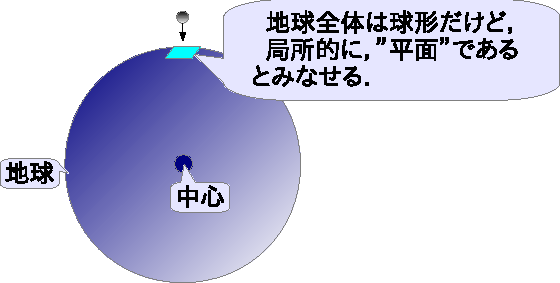
\includegraphics[keepaspectratio, width=6.5cm,height=4cm,clip]{ChiHyouHukin000.pdf}
                        \caption{地表付近は平面とみなしてよい}
                        \label{fig:HoubutsuSen}
                    \end{center}
                \end{figure}
            地球の重力加速度の方向は,常に物体から地球の中心へ向いている.
            地 とする.球表面付近では,重力加速度は鉛直下向きと近似できる
                \footnote{
                    「鉛直下向き」 とは,地表に垂直で,地表に向かう向きをいう.
                    鉛の球が重力で下向き(地球の中心に向かう向き)に引っ張られる
                    状況を描いたもの.物理学では,この表現がよく使われる.
                }.

            重力方向のみを考える場合,いちいち重力加速度をベクトル表記するのは
            面倒くさいし,読み手にしてみても式が煩雑で読みにくい.
            なので,重力加速度の向きが鉛直下向きであるという暗黙の了解をもたせて,
            方向の記述を省略することがほとんどである
                \footnote{
                    "省略" という言い方に躊躇するところがあるなら,
                    大きさのみに着目すると考えても同じことである.
                    要するに,重力加速度の定義の絶対値だけに着目して,
                    議論するということ.
                }.
            方向を省略すると,地球の重力加速度は
                \begin{equation*}
                    g = G\frac{M_{E}}{{r}^{2}}
                \end{equation*}
            となる.ここで,分母の ${|\br|}^{2}$ も,$r^{2}$ と略記した
                \footnote{
                    ベクトルを表す際の約束事として,ベクトル $\br$ の
                    大きさは,文字を細くして,$r$ と表す習慣がある.
                    細かいことを言うと,ベクトルの内積の公式のひとつに,
                    $\br\cdot\br = {\br}^{2} = |{\br}^{2}| = {|\br|}^{2} = r^{2}$
                    がある.
                }.

            さらに,ここで定義した地球の重力加速度に,地表からの高さ(いわば,標高)も
            組み込んで置きたい.方法は簡単で.地表からの高さを $h$ としたとき,
            $r$ に $r+h$ を代入してやればいい.
                \begin{align}
                    g = G\frac{M_{E}}{{(r+h)}^{2}}.
                \end{align}
            $r$ は地球の中心から地球表面までの距離である.
            地表からの高さを考慮したい場合は,地球の半径が大きくなったとして
            考えても同じ事で, $r$ に $h$ を加えるだけで済む.

            \begin{memo}{地表の重力加速度}
                地表なので,$h=0$として,計算しよう.
                地表の重力加速度 ${g}_{\mbox{地表}}$ は,
                \begin{align*}
                    {g}_{\mbox{地表}}
                    &= (6.673 \times 10^{-11}) \times
                        \frac{(5.974 \times 10^{24})}
                             {{(6.378 \times 10^{6})}^{2}} \\
                    %&= \frac{(6.673 \times 10^{-11}) \times (5.974 \times 10^{24})}
                    %         {{(6.378 \times 10^{6})}^{2}} \\
                    %&= \frac{39.864502 \times 10^{13}}{40.678884\times 10^{12}} \\
                    &= 9.799802275794 \\
                    &= 9.799  \,\mathrm{[m/s^{2}]} \quad \mbox{(有効桁数を考慮)}
                \end{align*}
                である.

                地球の重力加速度は大抵の場合,$g=9.80$[m/s] とされる.
                現実の地球は球形ではなく,楕円体である.だから,実際には地球の
                重力加速度は,場所ごとに違う.しかし,大まかな計算をする場合,
                $g=9.8$[m/s] として計算してよいだろう.

            \end{memo}

            \begin{memo}{エベレスト頂上の重力加速度}
                エベレスト頂上の標高は,8.848[km]であるという.
                なので,エベレスト頂上の重力加速度 ${g}_{\mbox{エベレスト頂上}}$ は,
                \begin{align*}
                    \mbox{}
                    &{g}_{\mbox{エベレスト頂上}} \\
                    &\quad = (6.673 \times 10^{-11}) \\
                    &\quad \quad \quad \times
                        \frac{(5.974 \times 10^{24})}
                             {{( (6.378 \times 10^{6}) + (8.848 \times 10^{3}) ) }^{2}} \\
                    %&= \frac{(6.673 \times 10^{-11}) \times (5.974 \times 10^{24})}
                    %         {{( (6.378 \times 10^{6}) + (8.848 \times 10^{3}) ) }^{2}} \\
                    %&= \frac{39.864502 \times 10^{13}}
                    %         {(40.678884 \times 10^{12})+(112.865088 \times 10^{9})+(78.287101 \times 10^{6})} \\
                    &\quad = 9.77266883...  \\
                    &\quad = 9.773 \,\mathrm{[m/s^{2}]} \quad \mbox{(有効桁数を考慮)}
                \end{align*}
                である.

                地表の重力加速度よりも小さい値となった.標高が $h=8.848$[km] の分,
                重力が弱まる.一般に,$h$ が大きいほど式の分母が大きくなり,重力が
                小さくなることは,容易にわかる.地球上で最大級の高さを誇る標高でも,
                $g=9.773$[m/s] で,$g=9.80$[m/s]と大差ない感じ
                    \footnote{
                        まあ,この差を大きいとみるか,小さいとみるかは,状況に
                        よるのだけど.
                    }.
            \end{memo}



%       %======================================================================
%       %  SubSection
%       %======================================================================
        \subsection{放物運動}
            \begin{mysmallsec}{概要}
            放物運動は,二次元的な(平面内の)運動である.つまり,2つの方向に対して
            運動方程式を考える必要がある.2方向として,垂直方向と水平方向を考える.
            ここで表現される水平とは,地上に対するものをいう.
            座標系は,垂直方向を $y$ とし,水平方向を $x$ とした直交座標とする.

            この2方向の運動は,互いに独立させて考えられる
                \footnote{
                    $x$ 方向の運動に,$y$ 方向の運動が影響することはない.逆も同じ.
                }.
            なので,垂直方向の運動と水平方向の運動を別々に考えた後,
            この2つの運動を重ねあわせることで放物物運動を見ていこう.
                \begin{figure}[hbt]
                    \begin{center}
                        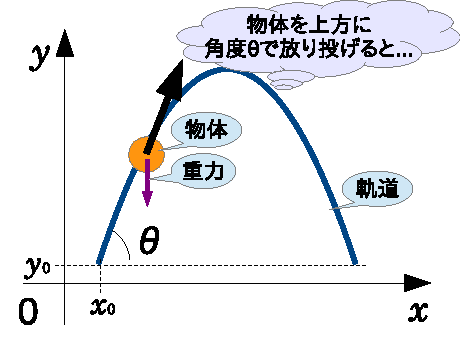
\includegraphics[keepaspectratio, width=6cm,height=6cm,clip]{HoubutsuSen.pdf}
                        \caption{放物運動}
                        \label{fig:HoubutsuSen}
                    \end{center}
                \end{figure}
            \end{mysmallsec}

            \begin{mysmallsec}{初期設定}
            初期設定を与えるところから,考察をはじめよう.
                \begin{itemize}
                    \item 開始時刻: $t=t_{0}$
                    \item 初期位置: ${\br}_{0} = \br(t_{0}) = (x(t_{0}),\, y(t_{0})) = (x_{0},\,y_{0})$
                    \item 初速度:  $\bv(t_{0})={\bv}_{0}$
                \end{itemize}
                        \begin{figure}[hbt]
                            \begin{center}
                                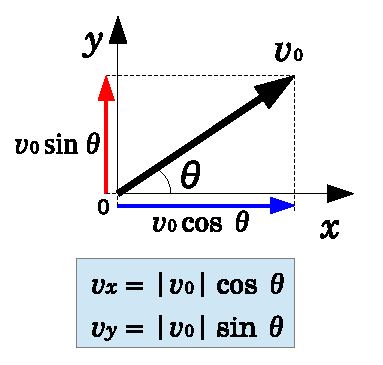
\includegraphics[keepaspectratio, width=6cm,height=6cm,clip]{HoubutsuSen_2.pdf}
                                \caption{放物運動開始}
                                \label{fig:HoubutsuSen}
                            \end{center}
                        \end{figure}

                初期条件から,垂直方向($y$ 軸方向)と水平方向($x$ 軸方向)の
                初速度$v_{x0},\,v_{y0}$ を求める.まず,図\ref{fig:HoubutsuSen}を
                みて,図形的イメージを覚えてもらいたい.やることは簡単で,
                三角関数を用いて,初速度 $\bv_{0}$ を $x$,$y$の各成分へ分解するだけだ.
                    \begin{align}
                        \mbox{(水平方向)} \quad v_{x0} &= |\bv_{0}| \cos \theta. \\
                        \mbox{(垂直方向)} \quad v_{y0} &= |\bv_{0}| \sin \theta.
                    \end{align}
            \end{mysmallsec}

            \begin{mysmallsec}{水平方向の運動方程式}
            水平方向の運動方程式の形は,
                \begin{equation*}
                    m\frac{{\df}^{2} x}{{\df t}^{2}} = F_{x}.
                \end{equation*}
            運動中は水平方向に力が働かないので,$F_{x} = 0$.よって,
                \begin{align}
                    m\frac{{\df}^{2} x}{{\df t}^{2}} = 0.
                \end{align}
            この方程式は,等速直線運動の方程式であり,以前に解いたことがある.
            速度は初速度のままで一定で,
                \begin{align}
                    v_{x}(t) = |\bv_{0}| \cos \theta
                \end{align}
            となる
                \footnote{
                    速度の関数に,独立変数として時間 $t$ を明示しているが,
                    左辺には時間は含まれいてない.これは時間に無関係であることを意味する.
                    しかし,ここではあえて,時間によらず一定であることを
                    示すために,時間を独立変数として記載することにしている.
                    理由は,垂直方向の速度は時間変化することと,対比したいからだ.
                }.
            位置は,
                \begin{align}
                    x(t) = v_{x}(t)t + x_{0} = (|\bv_{0}| \cos \theta)t +  x_{0}.
                \end{align}
            \end{mysmallsec}


            \begin{mysmallsec}{垂直方向の運動方程式}
                垂直方向の運動方程式は,
                    \begin{align}
                        m\frac{{\df}^{2} y}{{\df t}^{2}} = F_{y}.
                    \end{align}
                垂直方向は,重力が働いていることによる,等加速度運動である($F_{y}=-mg$)
                    \footnote{
                        1つ注意してほしい.重力加速度はベクトル量である.
                        だから,地球の重力加速度もベクトル表記して,$\bg$ と記述すべきだ.
                        だが,ここで考えているのは,垂直方向の1次元なので,ベクトル表記は
                        していない.
                    }.
                重力を運動方程式に代入し,整理しよう.
                    \begin{align*}
                        m\frac{{\df}^{2} y}{{\df t}^{2}} &= -mg \\
                         \frac{{\df}^{2} y}{{\df t}^{2}} &= -g. \quad(m \mbox{で両辺を割った})
                    \end{align*}
                等加速度運動についても,前に計算してあるので,ここではその結果を使う.
                加速度が $g$ の場合,等加速度運動の速度は,
                    \begin{equation*}
                        v_{y}(t) = -gt + v_{y0} = -gt + |\bv_{0}| \sin \theta.
                    \end{equation*}
                位置は,
                    \begin{equation*}
                        y(t) = -\frac{1}{2}g{t}^{2} + v_{y0}t + y_{0} = -\frac{1}{2}g{t}^{2} + (|\bv_{0}| \sin \theta)t + y_{0}.
                    \end{equation*}
            \end{mysmallsec}


            \begin{mysmallsec}{まとめ}
                以上の結果をまとめておこう.
                放物運動する物体の位置と速度は,
                \begin{align}
                                         \begin{bmatrix}
                                         x(t)   \\
                                         y(t)
                                 \end{bmatrix}
                            &=    \begin{bmatrix}
                                     (|\bv_{0}| \cos \theta)t +  x_{0}  \\
                                    -\frac{1}{2}g{t}^{2} + (|\bv_{0}| \sin \theta)t + y_{0}
                                 \end{bmatrix}.
                                 \\ \notag \\
                                                 \begin{bmatrix}
                                         v_{x}(t)  \\
                                         v_{y}(t)
                                 \end{bmatrix}
                            &=    \begin{bmatrix}
                                         |\bv_{0}| \cos \theta \\
                                         -gt + |\bv_{0}| \sin \theta
                                 \end{bmatrix}.
                \end{align}
            \end{mysmallsec}



%       %======================================================================
%       %  SubSection
%       %======================================================================
        \subsection{宇宙速度}
            宇宙空間で運動するために必要な速度のことを,
            \textbf{宇宙速度} という.
            宇宙速度とは,慣性運動のみで宇宙空間へ到達するために,
            最初に与える最低初速度をいう
                \footnote{
                    宇宙速度は,
                    宇宙空間に飛びたすために,絶対に書かせいない
                    速度ではない.地球の重力以上の力を対象物に与え続けられるのであれば,
                    どんなに遅くとも,宇宙空間に到達させることができる.
                    宇宙速度という概念は,慣性によって,宇宙へ到達するための初速度である.
                }.
            宇宙速度には3つの段階があって,
            それぞれ,\textbf{第一宇宙速度},\textbf{第二宇宙速度},
            \textbf{第三宇宙速度} とよばれる.
            各宇宙速度は,下のように定義される.
            \begin{description}
                \item[第一宇宙速度]\mbox{}\\
                    地表ギリギリで,等速円運動を続けるために必要な最小初速度.
                    地球と同じ大きさ,同じ質量の球体を地球に見立てて計算される値.
                    なので,空気抵抗や,建築物の有無は考慮しない.
                    地球の人工衛星になりたい場合に,必要な速度.
                \item[第二宇宙速度]\mbox{}\\
                    地球の重力を振り切り,地球圏外へ脱出するために必要な最小速度.
                    \textbf{脱出速度} といわれることも多い.
                    太陽の人工惑星になりたい場合に,必要な速度.
                \item[第三宇宙速度]\mbox{}\\
                    太陽圏外に脱出するために必要な最小速度.
                    太陽系にいるのが嫌になったときに,太陽系から脱出するために
                    は少なくともこの速度をもっていなければならない.
            \end{description}

        \subsubsection{第一宇宙速度}
            第一宇宙速度,要するに,地球の人工衛星になるために最低必要な速度,を計算しよう.
            何より最初に,運動方程式をたてよう.人工衛星になるためには,
            地球の周りを等速円運動しないといけない.人工衛星にしたい物体の速度を $v$ としたとき,
            半径 $R_{E}$ の地球の表面に軌道を描くには,万有引力と向心力を用いて,以下の方程式を
            満たす必要がある.向心力と万有引力は次の通り.
            \begin{align*}
                \mbox{(向心力)}   &= \frac{mv^{2}}{R_{E}+h}. \\
                \mbox{(万有引力)} &= G\frac{mM_{E}}{(R_{E}+h)^{2}}.
            \end{align*}
            よって,満たすべき方程式は,
            \begin{align}
                \frac{mv^{2}}{R_{E}+h} = G\frac{mM_{E}}{(R_{E}+h)^{2}}.
            \end{align}

            式を整理して,$v$ について解こう.
            \begin{align*}
                \frac{mv^{2}}{R_{E}+h} &= G\frac{mM_{E}}{(R_{E}+h)^{2}} \\
                v^{2} &= G\frac{M_{E}}{R_{E}+h}
            \end{align*}
            以上から,
            \begin{align}
                v = \sqrt{G\frac{M_{E}}{R_{E}+h}}. \quad (v<0\mbox{の解は除外})
            \end{align}

            $h=0$(地表すれすれを想定)のとき,上記の値 $G$,$M_{E}$,$R_{E}$ を
            代入してみよう.計算すると,
            \begin{align*}
                v &= \sqrt{(6.67 \times 10^{-11}) \times \frac{(5.97 \times 10^{24})}{(6.37 \times 10^{6})+0}} \\
                  &= \sqrt{\frac{6.67 \times 5.97}{6.37} \times  \frac{10^{-11} \times 10^{24}}{10^6{}}} \\
                  &= \sqrt{\frac{6.67 \times 5.97}{6.37} \times  10^{7}} \\
                  &= 7906.42 ...... \\
                  &= 7.91 \times 10^{3} \,\mathrm{[m/s]} \mbox{(有効桁数を考慮)}
            \end{align*}
            となった
                \footnote{
                    Python(2.7.3)を使って計算した.\sf{import math} で数学関数をインポートした後,
                    \sf{math.sqrt((6.67*5.97/6.37)*10**7)} を実行し,出力\sf{7906.428836995505} を得た.
                }.

            以上から,第一宇宙速度は,$7.91 \times 10^{3}$ [m/s] であることがわかった.


        \subsubsection{第二宇宙速度}
            第二宇宙速度は,地球の重力圏外に脱出するのに,最低限必要な初速度である.
            つまり,重力から生じる位置エネルギーを振り払うだけの速度(運動エネルギー)を
            与えてやらないといけない.言い換えると,
            運動エネルギーと地球の位置エネルギーの和が0以上
            になるように,初速度を与えるということだ
                \footnote{
                    重力による位置エネルギーは負であるから,合計が正になるような運動エネルギー
                    が必要とされる.
                }.

            地球の重力の位置エネルギー $U_{E}$ は
                \begin{equation*}
                    U_{E}=-G\frac{mM_{E}}{R_{E}+h}
                \end{equation*}
            である.ここで,上式は,地表から $h$ だけ上方の位置エネルギーを表している.
            よって,この位置エネルギー以上の運動エネルギーを与えればよい.
                \begin{equation*}
                    \frac{1}{2}mv^{2} + U_{E} \geq 0,
                \end{equation*}
            すなわち,
                \begin{align}
                    \frac{1}{2}mv^{2} - G\frac{mM_{E}}{R_{E}+h} \geq 0
                \end{align}
            を満たす $v$ であればよい.

            $v$ について解くと,
                \begin{align*}
                    \frac{1}{2}mv^{2} - G\frac{mM_{E}}{R_{E}+h} &\geq 0 \\
                    \frac{1}{2}v^{2}  - G\frac{M_{E}}{R_{E}+h}  &\geq 0 \\
                    \frac{1}{2}v^{2}                        &\geq  G\frac{M_{E}}{R_{E}+h} \\
                               v^{2}                        &\geq 2G\frac{M_{E}}{R_{E}+h} \\
                               v                            &\geq \sqrt{2G\frac{M_{E}}{R_{E}+h}}.
                \end{align*}
            最後の変形で,$v<0$ を除外した.第二宇宙速度は上式を満たす最小の $v$ であることから,
                \begin{align}
                    v = \sqrt{2G\frac{M_{E}}{R_{E}+h}}.
                \end{align}
            で計算できる.

            これに具体的な数値を代入してみよう($h=0$ として,地表すれすれを想定).すると,
                \begin{align*}
                    v &= \sqrt{2 \times (6.67 \times 10^{-11}) \times \frac{5.97 \times 10^{24}}{6.37 \times 10^{6}+0}} \\
                      &= \sqrt{\frac{2 \times 6.67 \times 5.97}{6.37} \times \frac{10^{-11} \times 10^{24}}{10^{6}}}    \\
                      &= \sqrt{\frac{2 \times 6.67 \times 5.97}{6.37} \times 10^{7}}   \\
                      &= 11181.37  ...... \\
                      &= 11.2 \times 10^{3} \,\mathrm{[m/s]}\mbox{(有効桁数を考慮)}
                \end{align*}
            となった
                \footnote{
                    Python(2.7.3)を使って計算した.\sf{import math} で数学関数をインポートした後,
                    \sf{math.sqrt((2*6.67*5.97/6.37)*10**7)} を実行し,出力\sf{11181.378891216778} を得た.
                }.

            以上から,第二宇宙速度は,$11.2 \times 10^{3}$ [m/s] であることがわかった.

            \begin{memo}{補足}
                第一宇宙速度と第二宇宙速度には,簡単な数値関係が知られている.というのも,
                    \begin{equation*}
                        \mbox{"第二宇宙速度"} = \sqrt{2}\mbox{"第一宇宙速度"}
                    \end{equation*}
                という関係があるのだ.実際に,
                \begin{align*}
                    \mbox{"第一宇宙速度"} \quad \sqrt{G\frac{M_{E}}{R_{E}+h}}  \\
                    \mbox{"第二宇宙速度"} \quad \sqrt{2G\frac{M_{E}}{R_{E}+h}}
                \end{align*}
                であり,
                    \begin{equation*}
                        \sqrt{2G\frac{M_{E}}{R_{E}+h}} = \sqrt{2} \sqrt{G\frac{M_{E}}{R_{E}+h}}
                    \end{equation*}
                が成立している.

                この規則を知っていると,第一宇宙速度と第二宇宙速度のどちらか一方が計算済みなら,
                他方を計算するのが楽になる.単に,$\sqrt{2}$ 倍,あるいは,$1/\sqrt{2}$ 倍すれば
                いいのだ.
            \end{memo}


        \subsubsection{第三宇宙速度}
            計算中.


    \subsection{躍度(jerk)と運動方程式}
        躍度$\bj$の定義式は以下であった\footnote{\ref{seq:jerk_define}節の式\eqref{eq:jerk_define}を参照.}.
        \begin{align*}
            \bj &:= \frac{\df \ba}{\df t} = \frac{{\df}^{3} \bx}{{\df t}^{3}}.
        \end{align*}

        これと運動方程式を関連づけてみよう.
        運動方程式は
            \[
                m\frac{{\df}^{2} \bx}{{\df t}^{2}} = \bF.
            \]
        であった.この式の両辺を時間微分すると,左辺に$\bj$が現れる.
        \begin{align*}
            m\frac{{\df}^{3} \bx}{{\df t}^{3}} &= \frac{\df \bF}{\df t}. \\
            \therefore \quad m\bj &= \frac{\df \bF}{\df t}.
        \end{align*}
        この式から,力の時間変化によって躍度(jerk)を発生させると解釈してよいだろう.

        人が物体を手で引っ張っている状況を想像してみると,常に正確に一定の力で引っ張ることは
        不可能である.機械に頼ったとしても,ブレはあるはず.
        それに,摩擦があることも想定できて,この場合は凸凹加減に場所によって物体にかかる合力
        が変わってくる.

        乗り物(車/電車/飛行機など)に乗っているとき,躍度が生じると不快感を感じる.
        車の停止状態からアクセルを踏む強さを急激に変えると,
        加速度が$\bzero$の状態から急に大きくなるため大きな躍度が生まれる.
        また,減速時もおなじである.等速直線運動していたとして,急にブレーキを踏めば,
        進行方向と逆向きの大きな加速度が生じる.

        躍度は実際には毎日ごく当たり前に感じている間隔を説明する大事な概念である.
        だけど,力学の教科書には躍度の紹介がないのはなぜだろうか.




    \subsection{円錐振り子}
    \begin{figure}[hbt]
        \begin{center}
            \includegraphicsdefault{ensui_furiko.pdf}
            \caption{円錐振り子}
            \label{fig:ensui_furiko}
        \end{center}
    \end{figure}

    \subsection{調和振動(単振動)}
    \subsubsection{弾性力}
        物体に対して,破壊しない程度の力を与えて,物体に歪を与えると,もとの形に戻ろうとする力が生じる.
        この力を \textbf{弾性力} という.

    \subsubsection{フックの法則}
        バネになんの力も加えられていない場合,その自然の長さを${l}_{0}$とする.
        バネの一端を固定し,他方を指でつまんで長さ$l$となるように力$\bF$で引っ張ってみる.
        このとき,バネからは縮もうとする向きに力が働く.このバネの力を$\bS$で表そう.
        $\bS$は弾性力の一種である.もとに戻ろうとする力というイメージから,\textbf{復元力} と
        もよばれる.
        バネを伸ばす力$\bF$と復元力$\bS$は互いに作用反作用の関係にある.よって,
        \begin{align}
            \bS = -\bF
        \end{align}
        の関係にある.

        \begin{figure}[hbt]
            \begin{center}
                \includegraphicsdefault{hookes_law.pdf}
                \caption{フックの法則}
                \label{fig:hookes_law}
            \end{center}
        \end{figure}
        バネの種類によって,その復元の力の置きさはことなる.
        その指標を \textbf{バネ定数} と名付けて,$k$とかくことにする.
        復元力の大きさは,バネの自然の長さからの変位$l-{l}_{0}$に比例することが知られていて,
        バネ定数$k$はこの比例定数である.式にすると,
        \begin{align}
            S = -k(l-{l}_{0})
        \end{align}
        である.ただし,バネが伸びる方を正の向きとする.バネが伸びるとき$S$は正の値をとり,
        バネが縮んでいるときは,$S$は負の値となる.自然の長さのとき,つまり,$l={l}_{0}$の
        場合は$S=0$であり,復元力は生じない.しかし,慣性の法則により,$S=0$のときにも運動
        は止まることはない.止まらなかった結果,バネが伸びる(あるいは縮む)ので,復元力が
        再び生じて延々と運動を繰り返す.

        バネの長さ$l$が自然長の長さ${l}_{0}$より長いとき(バネを引っ張っているとき)は
        \begin{align*}
                                      l  &> {l}_{0} \\
            \Leftrightarrow l - {l}_{0}  &> 0       \\
            \therefore S = -k(l-{l}_{0}) &< 0
        \end{align*}
        となり,$S$が負になるので,バネを引っ張る場合は縮む向きに復元力が働くことが式で
        表現できている.バネの長さ$l$が自然長の長さ${l}_{0}$より短いとき(バネを縮めているとき)は
        \begin{align*}
                                      l  &< {l}_{0} \\
            \Leftrightarrow l - {l}_{0}  &< 0       \\
            \therefore S = -k(l-{l}_{0}) &> 0
        \end{align*}
        となり,$S$が正になっていて,バネが伸びる向きに復元力が生じる.


    \subsubsection{単振動の種類}
        バネにくっついた物体が上下あるいは左右などに揺れている様子を \textbf{単振動} という.
        上下/左右ではなくても一方向の定常的な揺れであれば単振動である.摩擦などがあって徐々に振動が
        弱くなっていく場合は \textbf{減衰振動} という.物体がついていないもう片方の端っこ部分を
        振動させた場合は,\textbf{強制振動} という.教科書でよく例題として取り上げられるのは
        これくらいかな.
        \begin{figure}[hbt]
            \begin{center}
                \includegraphicsdefault{tanshindo_0.pdf}
                \caption{調和振動(単振動)}
                \label{fig:tanshindo_0}
            \end{center}
        \end{figure}


    \subsubsection{調和振動の運動解析}
    \begin{mysmallsec}{例題設定}
        バネ定数$k$のバネににつながった物体の動きを物理的に解析する.
        物体にかかる力は,重力$m\bg$とそれに対応する床からの垂直抗力$\bN$,バネから受ける弾性力$\bF$の3つである.
        今から考える状況はバネは水平にして,重力に対して垂直に運動するような場合を想定する.
        外力を与えない,バネのみの力による運動とする.図\ref{fig:tanshindo_1}にそのイメージを描く.
        図の上部が伸びが最大,図の下部が伸びが最小,それらの中間がバネが自然な長さにある瞬間を描いた.
        \begin{figure}[hbt]
            \begin{center}
                \includegraphicsdefault{tanshindo_1.pdf}
                \caption{調和振動の運動解析}
                \label{fig:tanshindo_1}
            \end{center}
        \end{figure}
    \end{mysmallsec}

    \begin{mysmallsec}{座標の設定}
        真横に振動する1次元の調和振動についての現象を解析するということだ.
        3次元座標のうち,$y$座標と$z$座標は常に0であるように座標を張ると,運動方程式が簡単になるので
            \footnote{
                教科書のような理想的な状況設定だと,調和振動は一方向のみの振動なので,
                全方向に成分を持つように座標を張ることは,座標設定ミスである.
                座標は計算しやすいように考えてから設定すべきだ.
            },
        物体の位置$\br$は次のように設定する.
        \begin{align}
            \br(t) = (x(t), \, y(t), \, z(t)) \left[= (x(t),\,0,\,0)\right].
        \end{align}
        ここで,カッコ$\left[\right]$でくくった部分$(x(t),\,0,\,0)$は次の初期値によって
        計算される結果であり,仮定ではない.逆に以下で,このようになるように,初期値を設定する.
    \end{mysmallsec}

    \begin{mysmallsec}{初期値}
        \begin{itemize}
            \item バネが自然の長さにあるときの物体の位置を${x}_{n}$とする

            \item $t=0$のときの物体の位置$\br(0)$を以下のようにとる
                  \begin{align}
                      \br(0) = (x(0), \, y(0), \, z(0)) := (x(0),\,0,\,0).
                  \end{align}
            \item 初速度$\bv(0)$はどの方向にも与えず,どの方向も0であるとする
                  \begin{align}
                      \bv(0) = ({v}_{x}(0), \, {v}_{y}(0), \, {v}_{z}(0)) := (0,\,0,\,0).
                  \end{align}
            \item 摩擦はなく,空気抵抗もなく,重力は至るところで均一で,外力も全く加えず,
                  電場や磁場もないし,当然,素粒子レベルの強い力や弱い力なんかは想定の範囲外
        \end{itemize}
    \end{mysmallsec}

    \begin{mysmallsec}{方向成分の解析(1):$y$成分と$z$成分}
        まず簡単な,$y$軸方向と$z$軸方向の運動を解析する.ここで設定した状況は,
        $y$方向へも$z$方向へも運動しない(位置を変えない)ように初期値設定と座標設定をしたはずである.
        そのことを確認しよう.

        バネから受ける弾性力$\bF$を成分表示すると,
            \begin{align}
                \bF = ({F}_{x}, \, {F}_{y}, \, {F}_{z}) = ({F}_{x},\,0,\,0).
            \end{align}
        となる.3次元ベクトルのまま考えてもよいが,この場合,$y$方向と$z$方向については位置の変化はない.
        例えば,$y$方向の位置と速度は,時間を独立変数として,位置を$y(t)$,速度を${v}_{y}(t)$とすると
        次のように計算される.
            \begin{align*}
                                m\frac{{\df}^{2} y(t)}{{\df t}^{2}}      &= {F}_{y}     \\
                \Leftrightarrow m\frac{{\df}^{2} y(t)}{{\df t}^{2}}      &= 0           \\
                \Leftrightarrow  \frac{\df}{\df t}\frac{\df y(t)}{\df t} &= 0           \\
                \therefore       \frac{\df y(t)}{\df t}                  &= {v}_{y}(0). \\
                \therefore      y(t)                                     &= {v}_{y}(0)t + y(0).
            \end{align*}
        初期値${v}_{y}(0):=0$,$y(0):=0$だから,
        \begin{align}
            y(t) = 0.
        \end{align}
        よって,$y$方向には微動だにしない.

        $z$軸方向も$y$軸方向と同じ条件なので,
        \begin{align}
            z(t) = 0.
        \end{align}
        である.
    \end{mysmallsec}

    \begin{mysmallsec}{方向成分の解析:(2)$x$成分}
        $x$軸方向にはバネの伸び縮みによる復元力が生じているので,
        フックの法則が使える.$x$方向に働く力${F}_{x}$は,バネ定数を$k$,
        バネの自然の長さを${x}_{n}$としたとき,
        \begin{align}
            {F}_{x} = -k(x(t)-{x}_{n})
        \end{align}
        で与えられる.よって,運動方程式は
        \begin{align}
            m\frac{{\df}^{2} x(t)}{{\df t}^{2}} = -k(x(t)-{x}_{n})
        \end{align}
        である.ここで,
        \begin{align}
            X(t) :=  x(t) - {x}_{0}
        \end{align}
        とおくと,
        \[
            \frac{\df X(t)}{\df t} = \frac{\df x(t)}{\df t} \, , \quad \frac{{\df}^{2} X(t)}{{\df t}^{2}} = \frac{{\df}^{2} x(t)}{{\df t}^{2}}
        \]
        であるから,
        \begin{align}
                            m\frac{{\df}^{2} X(t)}{{\df t}^{2}} &= -kX(t) \notag \\
            \Leftrightarrow \frac{{\df}^{2} X(t)}{{\df t}^{2}}  &= -\frac{k}{m}X(t)
        \end{align}
        となる.微分方程式を解くと,
        \begin{align}
                             X(t)            &= A \sin \sqrt{\frac{k}{m}} t + B \cos \sqrt{\frac{k}{m}} t \notag \\
            \Leftrightarrow  x(t) - {x}_{0}  &= A \sin \sqrt{\frac{k}{m}} t + B \cos \sqrt{\frac{k}{m}} t \notag \\
            \therefore       x(t)            &= A \sin \sqrt{\frac{k}{m}} t + B \cos \sqrt{\frac{k}{m}} t + {x}_{0}
        \end{align}
        を得る.角周波数$\sqrt{k/m}$を$\omega$でとおいてやると,見やすくなる.
        \begin{align}
            \omega := \sqrt{\frac{k}{m}}.
        \end{align}
        \begin{align}
            x(t) &= A \sin \omega t + B \cos \omega t + {x}_{0}.
        \end{align}

    \end{mysmallsec}

    \begin{mysmallsec}{結果}
        一次元の調和振動の解析結果.
        \begin{align}
            \br(t) &= (x(t),\,y(t),\,z(t)) \notag \\
                   &= (x(t),\,0,0)  \notag \\
                   &= (A \sin \omega t + B \cos \omega t + {x}_{0},\,0,\,0)
        \end{align}
    \end{mysmallsec}

